% -*- root: main.tex -*-
%-------------------------------------------------------------------------------
\chapterimage{chapter_head_9.pdf} 

%-------------------------------------------------------------------------------
\chapter{센서 정보 취득}

%-------------------------------------------------------------------------------
\section{USB 카메라}\index{USB 카메라}

%-------------------------------------------------------------------------------
\subsection{USB 카메라}\index{USB 카메라}

USB 카메라는 비디오 디바이스 중에 USB를 지원한다는 것을 의미한다. 다른 이름으로는 USB video device class 이라고 한다. 그래서 정칙 명칙은 UVC 카메라라고 해야 맞다고 볼 수 있다. 하지만, 본 강좌에서는 일반적으로 많이 사용되는 용어인 "USB 카메라" 이라고 칭하도록 하겠다. UVC는 현재 1.5버전까지 나왔으며 최신의 USB3.0 을 지원하며 리눅스, 윈도우즈, OSX 등 거의 모든 운영체제에서 사용가능하여 많이 사람들이 이용하고, 사용하기 편하고 수요가 많아서 다른 카메라에 비하여 저렴하게 나온것이 많다.

참고로, 웹캠이라고 부르는 경우가 있는데 이는 USB 카메라 혹은 USB를 지원하지 않는 카메라 중에 웹에 연결하여 사용할 수 있는 네트워킹 기능을 포함한 카메라도 있다. 흔히, LAN 및  Wifi 에 연결하여 웹상으로 데이터를 스트림하게 된다. 이 경우에 웹캠이라고 불러야 할 것이다. 그리고, 고속의 전송을 위한 FireWire (IEEE 1394규약) 를 이용하는 카메라도 있으며, 주로 고속으로 영상을 전송받아야하는 연구목적으로 많이 사용되고 있다. FireWire 규격은 일반적인 보드에서는 쉽게 찾아 볼 수 없으나 애플에서 개발하였기에 애플 제품에 많이 보게된다.

우리는 이 강좌를 통해 간단히 USB 카메라를 구동하고, 데이터를 확인하는 작업을 해보도록 하겠다.  USB 카메라를 이용한 얼굴 추적, 인식, 식별 및 다른 응용 프로그램은 추후에 다른 강좌를 통해 설명하도록 하겠다.

%-------------------------------------------------------------------------------
\subsection{관련 ROS 노드}\index{관련 ROS 노드}

ROS 에서는 USB 카메라와 관련하여 아래와 같은 다양한 패키지가 존재한다. 자세한 설명은 ROS 위키의 센서/카메라 에서 찾아볼 수 있다. 좌표는 http://wiki.ros.org/Sensors/Cameras 이다. 간략히 몇가지 패키지를 아래에 설명해 두었다.

\begin{description}
\item[libuvc-camera] UVC 표준을 사용하는 카메라들의 사용을 위한 인터페이스 패키지이다. (개발자: Ken Tossell)
\item[uvc-camera] 비교적 카메라 상세한 설정 변경이 있어 매우 편리하다. 더욱이 카메라 두대를 이용하여 스테레오 카메라를 이용할 수 있도록 할 수 있기에 스테레오 카메라를 생각하고 있다면 적정한 패키지가 아닐까 싶다.
\item[usb-cam] Bosch 에서 사용하는 매우 간단한 카메라 드라이버 (개발자:Benjamin Pitzer)
\item[freenect-camera]
\item[openni-camera]
\item[openni2-camera] 3가지 패키지 모두 카메라라는 명칭이 붙어 있지만 모두 Kinect 또는 Xtion과 같은 RGB-D 카메라를 위한 패키지들이다. 이들의 센서 역시 컬러 카메라를 포함하고 있기때문에 이들을 이용하려면 이 패키지들이 필요하다.
\item[camera1394] IEEE 1394 규격인 FireWire 를 이용하는 카메라를 위한 드라이버이다.
\item[prosilica-camera] 연구용으로 많이 사용되는 AVT사의 prosilica 카메라에 사용된다.
\item[pointgrey-camera-driver] 연구용으로 많이 사용되는 Point Grey Research사의 Point Grey 카메라를 위한 드라이버이다.
\item[camera-calibration] James Bowman, Patrick Mihelich가 개발한 카메라 캘리브레이션 관련 패키지로 OpenCV 의 캘리브레이션 기능을 응용한 패키지이다. 많은 카메라 관련 패키지가 이 패키지를 요구하는 경우가 있다.
\end{description}

%-------------------------------------------------------------------------------
\subsection{USB 카메라 테스트}\index{USB 카메라 테스트}

본 강좌에서는 Ken Tossell씨가 공개한 uvc-camera\footnote{http://wiki.ros.org/uvc\_camera}를 이용하기로 하겠다. 다른 관련 패키지도 거의 비슷한 사용방법이니 다른 패키지를 이용하고자 한다면 각 해당 패키지의 위키 페이지를 확인하도록 하자.

\setcounter{num}{0}

\vspace{\baselineskip}
\noindent
\stepcounter{num}\circled{\thenum} USB 카메라를 컴퓨터에 연결한다.
\stepcounter{num}\circled{\thenum} 카메라 정보를 확인한다.

\noindent
새로운 터미널을 하나 열고, 아래와 같이 "lsusb" 명령어로 접속이 제대로 되었는지 확인 가능하다. 일반적으로 UVC\footnote{http://en.wikipedia.org/wiki/USB\_video\_device\_class} 계열인 경우, 아무 문제 없이 아래의 빨간 메시지처럼 자신의 카메라를 확인할 수 있다. 

\begin{lstlisting}[language=ROS]
lsusb
Bus 002 Device 004: ID 1a40:0101 Terminus Technology Inc. 4-Port HUB
Bus 002 Device 003: ID 048d:1336 Integrated Technology Express, Inc. SD/MMC Cardreader
Bus 002 Device 002: ID 8087:0024 Intel Corp. Integrated Rate Matching Hub
Bus 002 Device 001: ID 1d6b:0002 Linux Foundation 2.0 root hub
Bus 006 Device 001: ID 1d6b:0003 Linux Foundation 3.0 root hub
Bus 001 Device 009: ID 0ac8:3420 Z-Star Microelectronics Corp. Venus USB2.0 Camera
Bus 001 Device 008: ID 0a12:0001 Cambridge Silicon Radio, Ltd Bluetooth Dongle (HCI mode)
Bus 001 Device 007: ID 046d:c52b Logitech, Inc. Unifying Receiver
Bus 001 Device 006: ID 1a40:0101 Terminus Technology Inc. 4-Port HUB
Bus 001 Device 005: ID 0853:0134 Topre Corporation 
Bus 001 Device 002: ID 8087:0024 Intel Corp. Integrated Rate Matching Hub
Bus 001 Device 001: ID 1d6b:0002 Linux Foundation 2.0 root hub
\end{lstlisting}

\stepcounter{num}\circled{\thenum} ROS uvc-camera 카메라 패키지 설치

\begin{lstlisting}[language=ROS]
sudo apt-get install ros-indigo-uvc-camera
\end{lstlisting}

\stepcounter{num}\circled{\thenum} ROS image 관련 패키지 설치

\begin{lstlisting}[language=ROS]
sudo apt-get install ros-indigo-image-*
sudo apt-get install ros-indigo-rqt-image-view 
\end{lstlisting}

\stepcounter{num}\circled{\thenum} uvc\_camera 노드 실행

uvc\_camera 노드를 실행하게 되면 [ WARN] [xxx]: Camera calibration 과 같이 카메라 캘리브레이션\footnote{http://wiki.ros.org/camera\_calibration}과 관련된 경고가 나오는데 특수한 경우가 아닌이상 본 강좌에서 다루려고 하는 범위에서는 해당되지 않는다. 일단, 무시해도 된다. 나중에 카메라 응용 강좌에서 카메라 캘리브레이션에 대해서 다루도록 하겠다.

\begin{lstlisting}[language=ROS]
$ roscore
$ rosrun uvc_camera uvc_camera_node
\end{lstlisting}

\stepcounter{num}\circled{\thenum} 관련 토픽 메시지 확인

아래와 같이 토픽 메시지를 보면 카메라 정보 (/camera\_info)와 이미지 정보 (/image\_raw)가 발신되고 있음을 확인할 수 있다.

\begin{lstlisting}[language=ROS]
$ $rostopic list
/camera_info
/image_raw
/image_raw/compressed
/image_raw/compressed/parameter_descriptions
/image_raw/compressed/parameter_updates
/image_raw/compressedDepth
/image_raw/compressedDepth/parameter_descriptions
/image_raw/compressedDepth/parameter_updates
/image_raw/theora
/image_raw/theora/parameter_descriptions
/image_raw/theora/parameter_updates
/rosout
/rosout_agg
\end{lstlisting}

%-------------------------------------------------------------------------------
\subsection{이미지 정보 확인}\index{이미지 정보 확인}

%-------------------------------------------------------------------------------
\subsubsection{image\_view 노드로 확인하기}

\setcounter{num}{0}

\noindent
\stepcounter{num}\thenum) 이미지 정보를 확인 할 수 있는 image\_view 노드를 실행하자.

\noindent
image:=/image\_raw 이라는 옵션이 붙는데, 맨뒤의 "/image\_raw" 라는 것은 좀 전에 토픽 리스트로 확인한 토픽을 이미지로 보기위한 옵션이다.

\begin{lstlisting}[language=ROS]
rosrun image_view image_view image:=/image_raw
\end{lstlisting}

\noindent
\stepcounter{num}\thenum) 아래의 그림과 같이 카메라의 이미지가 작은 윈도우창에 표시된다.

\begin{figure}[h]
\centering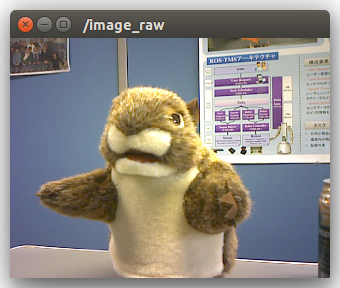
\includegraphics[width=0.5\columnwidth]{pictures/chapter9/imageview.png}
\caption{image\_view 노드를 이용한 이미지 보기}
\end{figure}

%-------------------------------------------------------------------------------
\subsubsection{RViz 로 확인하기}

\setcounter{num}{0}

\noindent
\stepcounter{num}\thenum) 시각화(visualization)툴인 RViz를 실행하자.

RViz 관련하여 더 자세한 사항은 "ROS 도구 (RViz)" 강좌를 참조하도록 하자.

\begin{lstlisting}[language=ROS]
rosrun rviz rviz
\end{lstlisting}

\noindent
\stepcounter{num}\thenum) Displays 옵션을 변경한다.

\vspace{\baselineskip}
\noindent
\thenum-1) Global Options → Fixed Frame 의 값을 "camera" 로 변경한다.

\vspace{\baselineskip}
\noindent
\thenum-2) RViz 왼쪽 하단의 "Add" 을 클릭하여 이미지 표시를 불러온다.

\noindent
(Add → by display → rviz → Image)

\begin{figure}[h]
\centering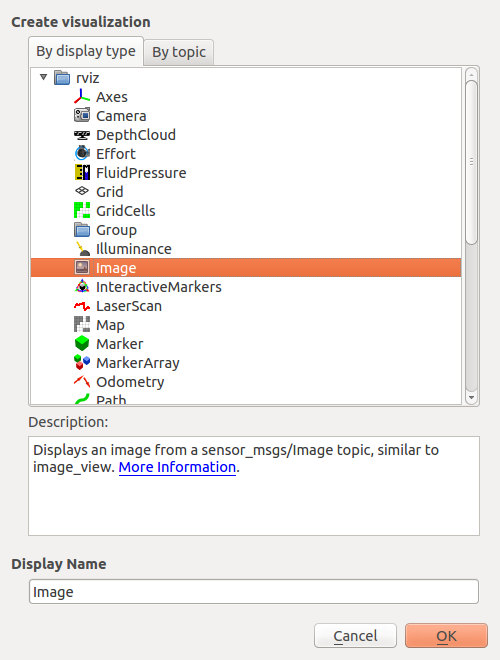
\includegraphics[width=0.5\columnwidth]{pictures/chapter9/add_display_of_rviz.png}
\caption{RViz에 이미지 디스플레이 추가}
\end{figure}

\vspace{\baselineskip}
\noindent
\thenum-3) Image → Image Topic 의 값을 "/image\_raw" 로 변경한다.

\begin{figure}[h]
\centering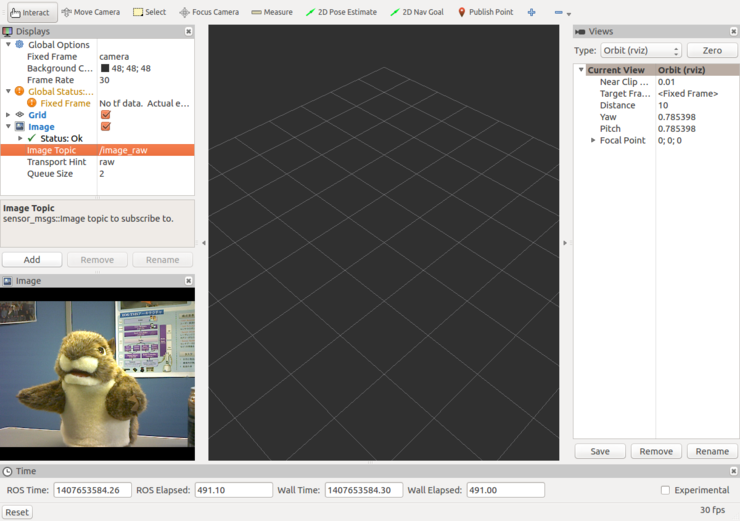
\includegraphics[width=0.9\columnwidth]{pictures/chapter9/rqt_image_full.png}
\caption{rqt를 이용한 이미지 확인}
\end{figure}

\vspace{\baselineskip}
\noindent
\thenum-4) 위 그림과 같이 Image 표시가 되게 된다.

%-------------------------------------------------------------------------------
\subsection{원격으로 이미지 전송}\index{원격으로 이미지 전송}

ROS 강좌를 처음부터 봤다면 위의 작업이 단일의 컴퓨터가 아니더라도 이미지 전송이 된다는 것을 알고 있을 것이다. 그 방법을 다시 간단히 설명하고, 원격의 컴퓨터인 카메라 접속된 컴퓨터 이외의 별도의 컴퓨터에서 이미지를 확인해보자.

%-------------------------------------------------------------------------------
\subsubsection{ROS 마스터 : 카메라가 연결된 컴퓨터}

ROS 마스터는 어떤 컴퓨터이든 상관 없지만 이번 강좌에서는 카메라가 연결된 컴퓨터가 ROS 마스터로 하였다. 아래처럼 네트워크 변수를 변경해주자. 아래의 예제의 IP 주소는 어디까지나 예제일뿐이다. 자신에게 맞는 아이피로 수정하자.

\begin{lstlisting}[language=bash]
export ROS_MASTER_URI=http://192.168.1.100:11311 
export ROS_IP=192.168.1.100
\end{lstlisting}

그 다음 ROS 마스터에서만 roscore를 구동해주고, uvc\_camera\_node 노드를 구동해 주면 된다.

\begin{lstlisting}[language=ROS]
roscore
rosrun uvc_camera uvc_camera_node
\end{lstlisting}

%-------------------------------------------------------------------------------
\subsubsection{원격 컴퓨터}

아래의 설정처럼 ROS 마스터를 카메라가 연결된 컴퓨터의 IP로 설정해주자. 그 다음에는 image\_view 만 구동해주면 된다.

\begin{lstlisting}[language=bash]
export ROS_MASTER_URI=http://192.168.1.100:11311 
export ROS_IP=192.168.1.120
\end{lstlisting}

\begin{lstlisting}[language=ROS]
rosrun image_view image_view image:=/image_raw
\end{lstlisting}

%-------------------------------------------------------------------------------
\section{레이저 레인지 파인더 (LRF)}\index{레이저 레인지 파인더 (LRF)}

%-------------------------------------------------------------------------------
\subsection{LRF (Laser Range Finder)}\index{LRF}

레이저 레인지 파인더 (Laser Range Finder\footnote{http://en.wikipedia.org/wiki/Laser\_rangefinder}), 흔히 LRF 로 불리우는 센서로서 레이저 스캐너(laser scanner), 광선 레이더(LIDAR) 라고도 불리우고있다. 고성능, 고속, 실시간 데이터 취득이라는 장점이 있기에 거리 측정을 이용한 활용 범위가 매우 넓다. 이러한 장점으로 로봇틱스 쪽도 매우 많이 사용되는 센서로, 거리 센서를 이용한 SLAM(Simultaneous localization and mapping\footnote{http://en.wikipedia.org/wiki/Simultaneous\_localization\_and\_mapping}), 물체 인식 및 사람 인식 등에도 사용되며, 실시간 성이 좋기 때문에 최근에는 무인자동차 등에도 많이 사용되고 있다. 

로봇쪽에서 많이 사용되는 대표적인 LRF으로는 실외용으로 무인자동차 등에 많이 사용되는 SICK\footnote{SICK, http://www.sick.com/}사의 LMS시리즈, 실내용으로 많이 사용되는 Hokuyo 의 URG 시리즈\footnote{URG 시리즈, https://www.hokuyo-aut.jp/products/}, 그리고, 레이저를 복수개 탑재한 Velodyne의 HDL 시리즈\footnote{http://velodynelidar.com/lidar/lidar.aspx}가 있다. 그리고 각 회사 등에서는 대표제품 이외에도 3D 를 위한 복수개의 레이저를 탑재한 센서등이 활발하게 개발 중에 있다.

이러한, 센서들의 가장 큰 문제점은 가격이다. 기본적인 가격은 제품마다 다르겠지만 수 백만원대이고, Velodyne의 HDL시리즈의 경우에는 수 천만을 호가하는 제품들이다. 이러한 단점을 커버하기 위한 중국 제품 (RPLIDAR\footnote{http://www.robopeak.com/} 등) 등이 40만원 안밖으로 저가로 나오기 시작하였으니 앞으로 더 기대해 볼 만 하다고 볼 수 있다.

\begin{figure}[h]
\centering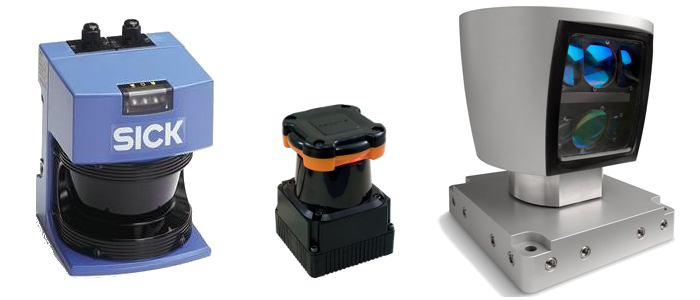
\includegraphics[width=0.7\columnwidth]{pictures/chapter9/sickhokuyovelodyne.png}
\caption{왼쪽: SICK LMS 210, 가운데 Hokuyo UTM-30LX, 오른쪽: Velodyne HDL-64e}
\end{figure}

%-------------------------------------------------------------------------------
\subsection{LRF 측정 원리}\index{LRF 측정 원리}

\begin{equation}
  D = \frac{1}{2}ct = \frac{1}{2}\frac{c\varphi}{\omega} = \frac{c}{4\pi f}(N\pi +  \Delta\varphi) = \frac{\lambda}{4}(N +  \Delta N)
\end{equation}

위 식\footnote{\url{http://en.wikipedia.org/wiki/Laser_rangefinder}}에서 사용된 정의는 이와 같다. $c$ 광원의 속도, $t$ 반사되어 돌아온 시간, $\varphi$ 위상 딜레이, $\omega$ 광파의 각주파수, $\lambda$ 파장, $N$ 파장 반주기. 여기서 사용자는 레이저가 돌아온 시간을 반으로 나누어 거리를 계산한다고 보면 된다.

문제는, 여기서 사용되는 레이저는 제어 및 가격의 문제로 적게 쓸수록 이득이기에 제조 회사들은 레이저 광원을 하나만 사용하게 된다. 참고로 수 천만원 이상의 Velodyne의 HDL시리즈는 적게는 32개, 많게는 64개의 레이저를 사용하고 있다. 그 이외에는 대부분 하나의 레이저를 사용한다고 보면 된다. 

이런 문제를 극복하기 위하여, LRF 는 하나의 레이저와 하나의 반사거울과 모터로 구성되어 있다. LRF 를 구동하면 모터 소리가 들리는데 이는 내부의 거울을 회전시켜서 레이저를 수평면으로 주사하기 때문이다. 제품마다 다르겠지만 일반적으로 180도~360도 까지 측정 가능하다. 

밑에 그림에서 (a)는 LRF 의 모습으로 내부에 레이저가 하나 있고, 이를 거울(회색부분)을 회전시켜가며 레이저의 반사되어 온 시간을 측정하게 된다 (엄밀히 말하면 파장계산이지만...). 이렇게 하여 그림 (b)와 같이 LRF 를 중심으로 수평면의 물체들을 스캔 가능하다. 다만, 단점으로는 거리가 멀어짐으로써 정확도가 떨어짐을 알 수 있다. (그림 (c))

\begin{figure}[h]
\centering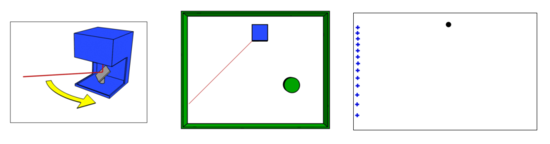
\includegraphics[width=0.8\columnwidth]{pictures/chapter9/mechanism_lrf.png}
\caption{LRF 측정 원리}
\end{figure}

사용자 입장에서 LRF 의 동작 원리는 굳이 알 필요는 없다. 여기서 이 내용을 포함한 이유는, 이 원리로 인하여 측정할때 주의할 점이 있다는 점이다. 

첫째, 레이저를 광원으로 사용하고 있기 때문에, 강한 레이저 빔으로 눈을 손상시킬 수 있다. 단, 제품마다 틀린데 등급을 나누고 있으므로 제품을 구입할 때 참고해야할 중요한 사항이다. 일반적으로 레이저 등급\footnote{http://www.ipgphotonicskorea.com/company\_service\_safety.htm}은 Class 1에서 Class 4까지 나뉘고 있고 숫자가 높아질 수록 위험하다는 의미이다. 클래스1의 경우에는 안전한 제품으로 직접 눈에 닿아도 문제 없는 등급이고, 클래스 2부터는 장기간 노출시 위험이 높아진다. 위에서 설명한 LRF 의 경우, 클래스 1에 해당된다.

둘째, 레이저 광원이 반사되어 돌아오는 것을 측정하기 때문에 반사되지 않으면 소용이 없다. 즉, 투명한 유리, PET 병, 유리컵 등은 반사되지 않고 투과하거나 산란된다. 그리고, 거울의 경우에는 재반사되므로 정확한 값을 얻을 수 없다.

셋째, 수평면을 주사하기 때문에 센서를 기준으로 수평면 상의  물체만 검출된다. 즉 2D 데이터임을 알아야 한다. (일부, LRF의 경우 센서 자체를 회전시켜 3D 로 측정하는 경우도 있음.)

%-------------------------------------------------------------------------------
\subsection{LRF 연결 및 테스트}\index{LRF 연결 및 테스트}

ROS 에서는 SICK 사의 LRF지원하는 sicks300, sicktoolbox, sicktoolbox\_wrapper 패키지, Hokuyo 사의 LRF를 지원하는 hokuyo\_node\footnote{http://wiki.ros.org/hokuyo\_node}, urg\_node\footnote{http://wiki.ros.org/urg\_node} 패키지, velodyne 사의 LRF를 지원하는 velodyne 패키지 등이 있다.

이 중에서, 본 강좌에서는 Hokuyo 사의 UTM-30LX\footnote{https://www.hokuyo-aut.jp/02sensor/07scanner/utm\_30lx.html} 를 사용하여 테스트할 예정이기에 urg\_node 패키지를 이용하기로 하겠다. 참고로 Hydro 이전에는 hokuyo\_node를 많이 사용했지만 새로운 통신 기준까지 지원하는 urg\_node가 메인 패키지로 되었다.

%-------------------------------------------------------------------------------
\subsubsection{urg-node 패키지 설치}

\begin{lstlisting}[language=ROS]
sudo apt-get install ros-indigo-urg-node 
\end{lstlisting}

%-------------------------------------------------------------------------------
\subsubsection{디바이스 사용권한 변경}

LRF를 컴퓨터에 접속하도록 하자. USB 방식이므로 USB포트에 삽입만 하면 된다. 그 뒤, ttyACMx 으로 인식되기에 아래와 같이 권한 설정을 하도록 하자. (참고로 본 강좌에서는 ttyACM0 으로 인식 되었다.)

\begin{lstlisting}[language=ROS]
$ cd /dev
$ ls -l ttyACM*
crw-rw---- 1 root dialout 166, 0 Aug 11 14:30 ttyACM0
\end{lstlisting}

위 결과를 보면 ttyACM0 의 권한이 주어지지 않았다. chmod 명령어로 권한을 설정해 주도록 하자.

\begin{lstlisting}[language=ROS]
$ sudo chmod a+rw /dev/ttyACM0
$ ls -l ttyACM*
crw-rw-rw- 1 root dialout 166, 0 Aug 11 14:35 ttyACM0
\end{lstlisting}

chmod 명령어로 권한이 변경되었음을 확인할 수 있다.

%-------------------------------------------------------------------------------
\subsubsection{urg-node 노드 실행}

본 강좌 부터는 roscore는 실행되어 있다는 전제로 설명하겠다. roscore 설명은 섹션~\ref{subsec:Roscore}~\nameref{subsec:Roscore}(pp.\pageref{subsec:Roscore})를 참고하기 바란다.

\begin{lstlisting}[language=ROS]
rosrun urg_node urg_node 
\end{lstlisting}

%-------------------------------------------------------------------------------
\subsubsection{urg-node 노드에서 발행되는 /scan 데이터 확인}

urg-node 노드를 실행하게 되면 /scan 이라는 토픽으로 LRF 값이 전송된다. 아래와 같이 값을 확인해 보자. 

\begin{lstlisting}[language=ROS]
$ rostopic echo /scan
header: 
  seq: 5866
  stamp: 
    secs: 1407735556
    nsecs: 501421233
  frame_id: laser
angle_min: -2.35619449615
angle_max: 2.35619449615
angle_increment: 0.00436332309619
time_increment: 1.73611151695e-05
scan_time: 0.0250000003725
range_min: 0.0230000000447
range_max: 60.0
ranges: [0.9929999709129333,1.3346457658567, .............................
\end{lstlisting}

위와 같이 스캔 정보를 확인할 수 있다. frame\_id는 laser로 설정되어 있고, 측정각은 -(2.35619449615 radians) = -135 degree 이기때문에 최소 -135도, 최대 135도 이기 때문에 총 270도 측정 범위임을 확인할 수 있다. 또한, 각 증가값은 0.25° (270도를 측정할때 1,440 steps 번 측정한다) 이고, 270도를 한번 스캔하는데 총 25msec 가 소요 된다는 것도 알 수 있다.

%-------------------------------------------------------------------------------
\subsection{LRF 거리 정보값 확인}

%-------------------------------------------------------------------------------
\subsubsection{RViz 실행}

\begin{lstlisting}[language=ROS]
$ rosrun rviz rviz
\end{lstlisting}

%-------------------------------------------------------------------------------
\subsubsection{Displays 옵션 변경}

1) Fixed Frame 변경
Global Options → Fixed Frame 을 laser 로 변경한다.

2) Axes 추가 및 설정
rviz 좌측 하단의 Add 클릭한 후, Axes 선택하여 추가한다.
아래 그림과 같이 세부 설정을 바꿔준다. (Length 및 Radius)

3) LaserScan 추가 및 설정
rviz 좌측 하단의 Add 클릭한 후, LaserScan 선택하여 추가한다.
아래 그림과 같이 세부 설정을 바꿔준다. (Topic 및 Color Transformer, Color)

\begin{figure}[h]
\centering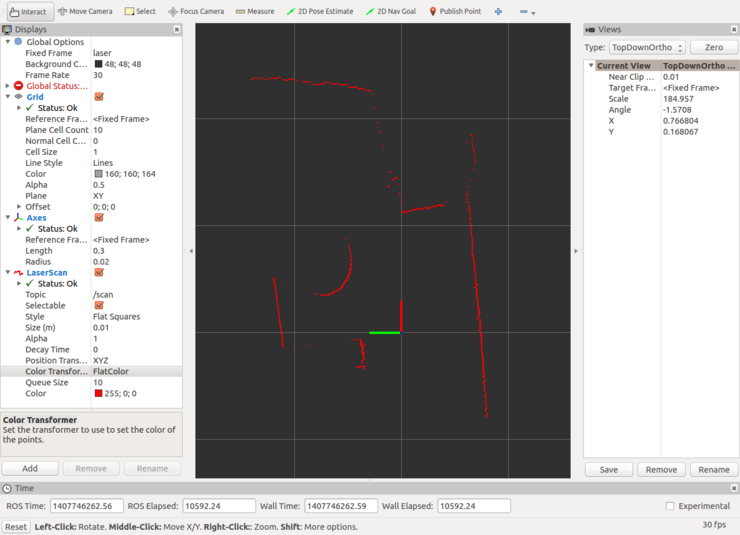
\includegraphics[width=0.9\columnwidth]{pictures/chapter9/rviz_laser_scan.png}
\caption{RViz에 LaserScan 디스플레이}
\end{figure}

%-------------------------------------------------------------------------------
\subsubsection{데이터 확인}

위 그림과 같이, 가운데 빨간색과 녹색으로 된 축을 중심으로 주변의 물체가 스캔되어 점으로 표현되어 있다는 것을 확인 할 수 있다. 회색 격자가 1미터로 설정되어 있기 때문에 실제 상황과 매치되어 확인 할 수 있다.

%-------------------------------------------------------------------------------
\subsection{LRF 활용}

LRF 활용은 무궁무진 할테지만 대표적인 예는 SLAM (Simultaneous localization and mapping) 이라고 할 수 있다. 아래의 그림과 같이 로봇에 LRF 를 장착하고, 로봇을 중심으로 장애물을 인식하고 맵을 작성하며 나아가는 것이다. 이 부분에 대해서는 추후에 강좌를 통해서 소개하도록 하겠다.

LRF 의 또다른 예로는 아래의 동영상과 같이 환경에 있는 다양한 물체인식과 사람의 발 혹은 몸체를 측정하여 위치를 추척하고 주변의 상황과 매치하여 현재 행동을 추리하는 것도 가능하다. 필자의 석사 연구 테마였는데 올해 가을경에 관련 소스를 오픈할 준비를 하고 있다. 그 때에 관련 응용 강좌를 준비하도록 하겠다.

그 이외에도 아래의 동영상처럼 2D의 LRF 센서 몸체 자체를 회전시켜 3차원 정보를 생성, 3D 환경 지도를 작성할 수 도 있다. 필자의 연구\cite{pyo2014floor}에서는 이러한 부분도 다루고 있으니 이 부분에 대해서도 다루고 싶다.

\begin{figure}[h]
\centering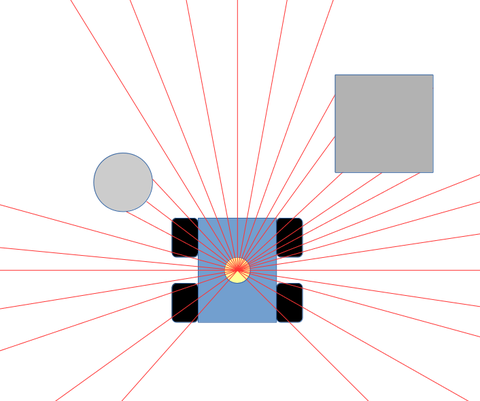
\includegraphics[width=0.5\columnwidth]{pictures/chapter9/lrfandrobot.png}
\caption{LRF 활용1: 모바일 로봇의 장애물 검출}
\end{figure}

\begin{figure}[h]
\centering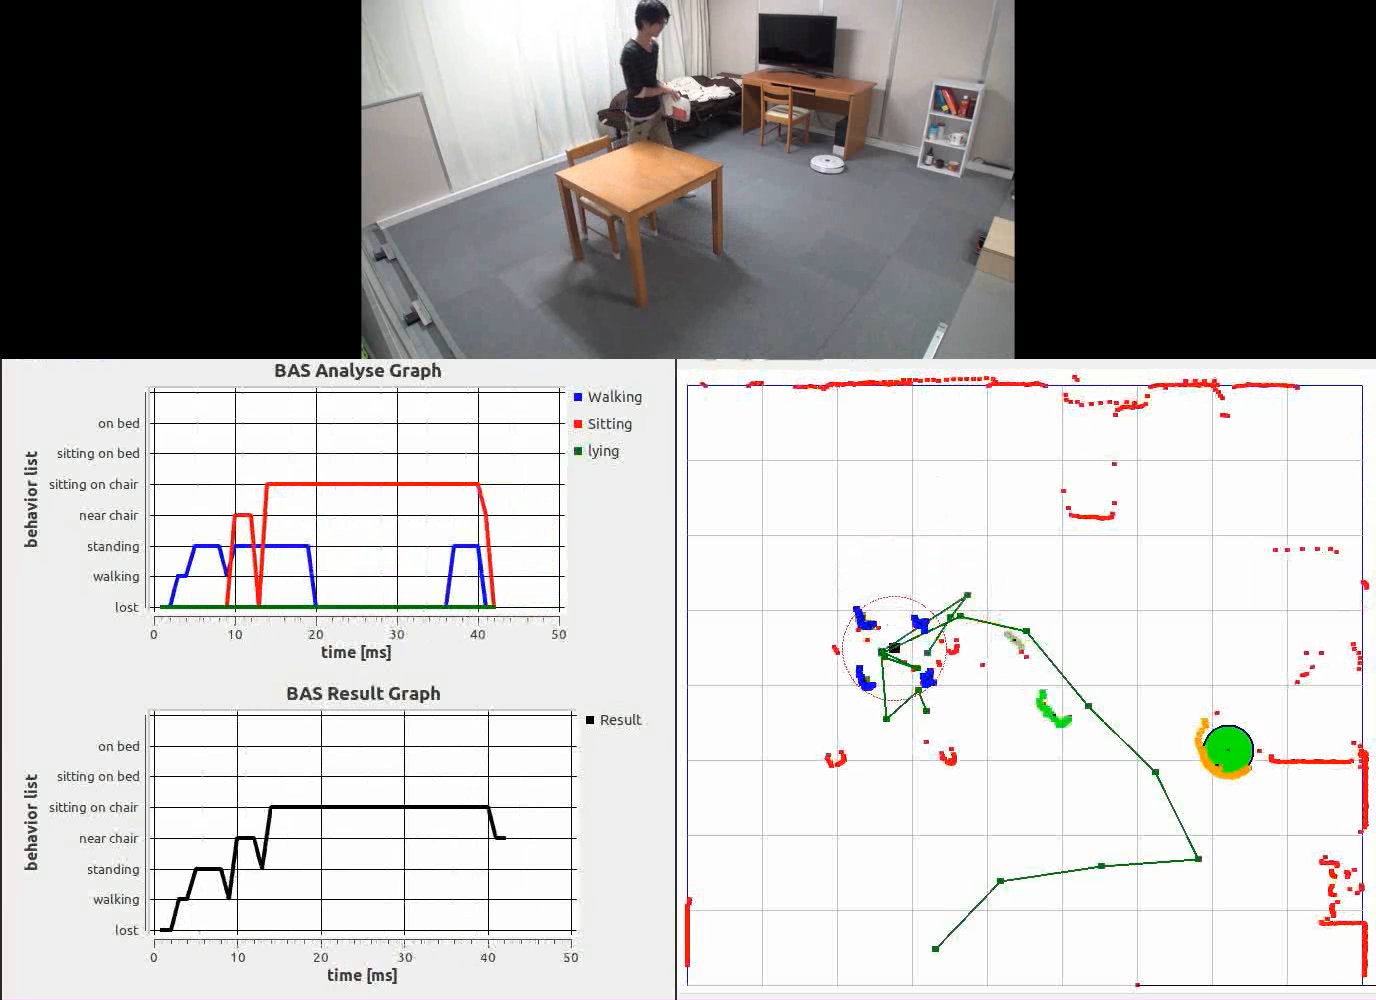
\includegraphics[width=0.7\columnwidth]{pictures/chapter9/fss.png}
\caption{LRF 활용2: 인물 및 이동 물체 검출}
\end{figure}

%-------------------------------------------------------------------------------
\section{Depth Camera}\index{Depth Camera}

%-------------------------------------------------------------------------------
\subsection{Depth Sensor}\index{Depth Sensor}

Depth camera 를 우리말로 치면 깊이 카메라 정도로 받아 드릴 수 있다. 이 이외에도 LRF 와 같은 범주에서 Depth sensor 라고도 불리우고, 컬러 영상과 함께 취득할 수 있는 경우에는 RGB-D camera, MS사에서 대중화에 성공시킨 의미에서 Kinect Camera 등 다양하게 불리우고 있다. 본 강좌에서는 용어가 헤깔리지 않도록 Depth camera 라고 칭하겠다.

Depth camera 에는 그 취득 방법에 따라 매우 다양한 종류로 나뉠 수 있는데, 그 중 대표적으로 ToF(Time of flight)\footnote{ToF, http://en.wikipedia.org/wiki/Time\_of\_flight} 와 일관적 방사 패턴(pattern of coherent radiation, US20100225746 특허 인용) 으로 나눌 수 있다.

ToF 방식은 적외선을 방사하여 돌아온 거리로 거리를 측정하는 방식으로 일반적으로는 IR 송신부와 수신부가 쌍으로 존재하여(적외선 카메라를 사용하는 제품등, 제품에 따라 다른 경우도 있음) 각 픽셀에서 측정한 거리를 읽어내는 방식이다. ToF 방식이 다음에 설명할 일관적 방사 패턴 방식보다 비싼 이유는 이러한 구조적인 면에서 하드웨어가 가격이 올라가기 때문이다 (최근에는 위상차를 이용한 거리계산등 다양한 방법이 소개되어 가격이 낮아지고 있는 추세이다). ToF 방식\footnote{ToF Camera, http://en.wikipedia.org/wiki/Time-of-flight\_camera}의 센서로는 파나소닉의 D-IMager, MESA Imaging사의 SwissRanger, Fotonic 사의 FOTONIC-B70, pmdtechnologies 사의 CamCube와 CamBoard, SoftKinectic사의 DepthSense DS시리즈, MS사의 최근에 출시한 Kinect 2 등이 있다.

\begin{figure}[h]
\centering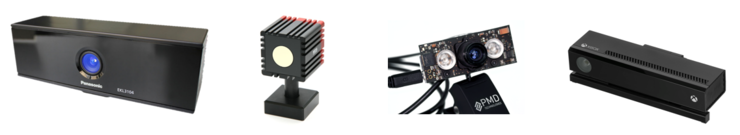
\includegraphics[width=0.9\columnwidth]{pictures/chapter9/tof.png}
\caption{왼쪽부터 D-IMager, SwissRanger, CamBoard, Kinect2}
\end{figure}

일관적 방사 패턴 방식(pattern of coherent radiation, US20100225746\footnote{http://www.google.com/patents/US20100225746} 특허 인용, 가간섭성 방사라고도 한다.)의 경우에는 많이 들어본 MS사의 Kinect\footnote{Kinect, http://en.wikipedia.org/wiki/Kinect}와 Asus 의 Xtion\footnote{http://www.asus.com/Multimedia/Xtion\_PRO\_LIVE/} 이 있다. 그 이외에도 PrimeSense사의 Carmine, Capri 등이 있고, 최근에는 occipital 사의 structure sensor\footnote{structure sensor, http://structure.io/}가 출시 되었다. 이들 센서들의 공통점은 PrimeSense 사의 PrimeSense System on a Chip (SoC) 을 사용하고 있다는 것이다. 

\begin{figure}[h]
\centering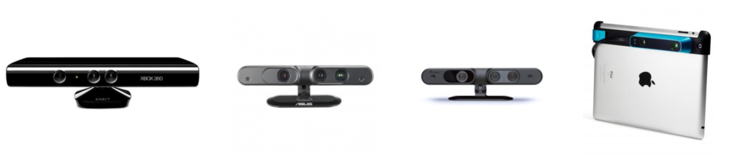
\includegraphics[width=0.9\columnwidth]{pictures/chapter9/pattern.png}
\caption{왼쪽부터 Kinect xbox, Xtion, Carmine}
\end{figure}

PrimeSense 사의 단 하나의 적외선 프로젝터와 단 하나의 적외선 카메라로 구성된 센서로, 기존 ToF 방식에서는 없었던 "일관적 방사 패턴"을 사용한다는 점이다. 이는 미국 특허 US20100225746 에 자세히 기재되어 있다. 또한, 이 기술을 집접시킨 PrimeSense System on a Chip (SoC) 도 개발되었다. 

간단히 소개하자면, 밑의 그림중 26번에 해당되는 프로젝터가 랜덤하게 적에선 점들을 일정한 패턴에 의해 적외선 점들을 방사하게 된다. 방사된 적외선 점들은 31번과 같이 대상체에 투영되고, 이 점들을 적외선 카메라인 32번에 의해서 수집하게 되는 것이다. 여기서 31번의 무수한 일정 패턴의 적외선 점들은 평평한 대상체라면 패턴들이 방사된 시점에서 동일하겠지만 장애물이 놓여지게 되면 일그러지게 되고 변형된다. 그 예가 그림 \ref{fig:irpattern}\footnote{\url{https://www.youtube.com/watch?v=Tpa1JP1AtCo}}와 같다. 이 변형을 적외선 프로젝터와 적외선 카메라의 거리를 가지고 수학적 계산으로 풀게되면 거리를 계산할 수 있게 된다.

\begin{figure}[h]
\centering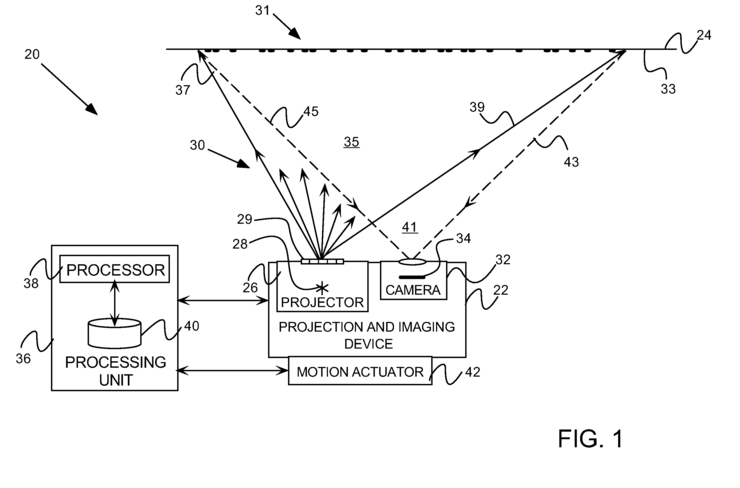
\includegraphics[width=0.8\columnwidth]{pictures/chapter9/US20100225746A1_20100909_D00001.png}
\caption{미국 특허출원번호 US20100225746 에 기재된 적외선 프로젝터}
\end{figure}

\begin{figure}[h]
\label{fig:irpattern}
\centering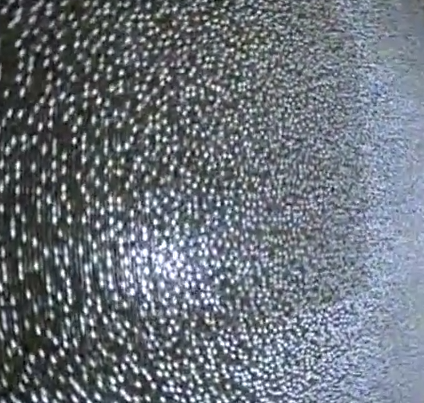
\includegraphics[width=0.4\columnwidth]{pictures/chapter9/irpattern.png}
\caption{Kinect 의 IR 패턴을 찍은 사진}
\end{figure}

이 기술은 기존의 ToF 방식을 지원하는 하드웨어가 비싸다는 문제점과 외부 간섭등의 문제점을 해결하면서 관심을 받게 되었고, PrimeSense 사의 PrimeSense SoC 를 탑재한 자사의 Carmine, Capri 가 세상에 나왔다. 또한 같은 SoC칩을 탑재한 MS 사의 Kinect 의 경우에는 Xbox 의 컨트롤러로 대중화되면서 인기를 한 몸에 받을 수 있었다. 그 뒤로도 일반 PC에서의 사용을 염두해둔 Asus의 Xtion 등이 나올 수 있었다. 이는 모두,  PrimeSense SoC 를 탑재한 센서들이다. 단, 문제는 2013년 12월 PrimeSense 사가 Apple 사에 인수되면서 발생되었다. PrimeSense 사가 Apple 사에 인수된 이후, PrimeSense의 Carmine, Capri 제품을 구매할 수 없게된 것은 물론, MS사의 Kinect는 판매중지가 되었고, Asus의 Xtion 또한 재고품을 제외한 추후 생산을 중단하게 되었다. PrimeSense SoC 를 탑재한 마지막 제품인 Occipital 사의 Structure sensor 는 현재까지 제품을 판매하고 있지만, 추후 어떻게 될지는 당사도 모르는 분위기이다. 저렴한 가격으로 인기를 끌었던 한 제품이 역사속으로 숨어버리게 된 상황이다. 하지만, 앞으로 구글의 Tango 프로젝트 및 Apple사의 PrimeSense 사 인수후 나올 제품, ToF 계열의 Canesta 사를 인수한 MS사의 후속 제품인 Kinect 2 등이 기대되어지는 상황이다.

%-------------------------------------------------------------------------------
\subsection{OpenNI (Open Natural Interaction)}\index{OpenNI}

OpenNI (Open Natural Interaction)\footnote{OpenNI, http://en.wikipedia.org/wiki/OpenNI}란 PrimeSense 사를 중심으로 Willow Garage, ASUS와 함께 개발한 자사의 제품들을 사용하기 위해 개발한 드라이버와 다양한 응용 API의 집합의 라이브러리이다. 여기서 NI는 Natural Interaction의 약자로, 인간과 기계의 의사소통이라는 뜻으로 키보드 마우스 등이 아닌 인간의 감각을 기본으로한 상호작용이라는 의미에서 나왔다. PrimeSense SoC 를 탑재한 대부분의 센서는 이 드라이브를 사용하고 있다. 비슷한 형태의 MS사의 Kinect Windows SDK 및 한 때 MS사의 Kinect를 처음 해킹하여 프리로 내놓았던 것으로 유명한 libfreenect 등이 있다. OpenNI에는 Ponit Cluoud Data를 다루는 기본적인 드라이버 이외에 사람의 인체 골격을 다루는 NITE 등의 미들웨어도 포함되어 있다. OpenNI 는 PrimeSense 이 Apple 사로 인수된 후, 폐기의 위기에 놓였다가, 현재는 Occipital 사가 뒤를 이어 Github 저장소\footnote{\url{https://github.com/occipital/openni2}}에서 개발을 이어가고 있다.

%-------------------------------------------------------------------------------
\subsection{점 군 데이터 (Point Cloud Data) 와 Point Cloud Library}\index{PCL}

방식의 차이에 따라 Depth Sensor 의 경우, LRF와 Depth Camera 로 나뉘기도 하는데, 이 범주의 모든 거리 센서등은 대상체와의 거리를 한 점으로 표시하고 이를 점들의 집합체인 Point Cloud 를 다룬다는 의미에서 동일하다. OpenNI 또한 Point Cloud 를 만들어 낸다. 이러한 Point Cloud 를 사용하기 위한 API 의 잡합체로 우리는 PCL (Point Cloud Library)\footnote{PCL, http://pointclouds.org/about/} 이라는 라이브러리를 사용한다. PCL 은 그 기능이 많아 다 설명하기 어렵지만 PCL 사이트에 대표적인 특징이 있는 사진이 있어서 첨부한다. 아래의 그림과 같이 PCL 에서는 점 군 데이터(PCD) 을 가지고 아래의 그림\footnote{\url{http://www.pointclouds.org/}}처럼 필터링, 분할, 표전 재구성, 모델로부터의 피팅 및 특징 추출 등을 행하는 라이브러리이다. 거의 모든 PCD 를 이용한 처리에 필요한 함수등을 가지고 있다. 우리는 나중에 이 PCL 을 이용하여 PCD 를 처리할 예정이다.

\begin{figure}[h]
\centering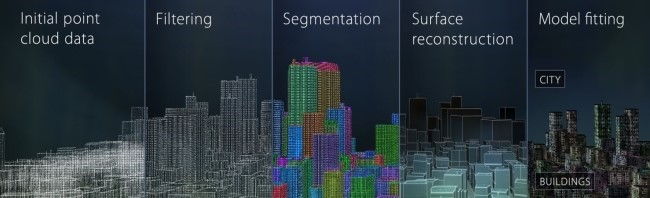
\includegraphics[width=0.9\columnwidth]{pictures/chapter9/pcl_features.jpg}
\caption{PCL 특징}
\end{figure}

%-------------------------------------------------------------------------------
\subsection{Depth camera 의 드라이버 설치 및 구동}

\begin{figure}[h]
\centering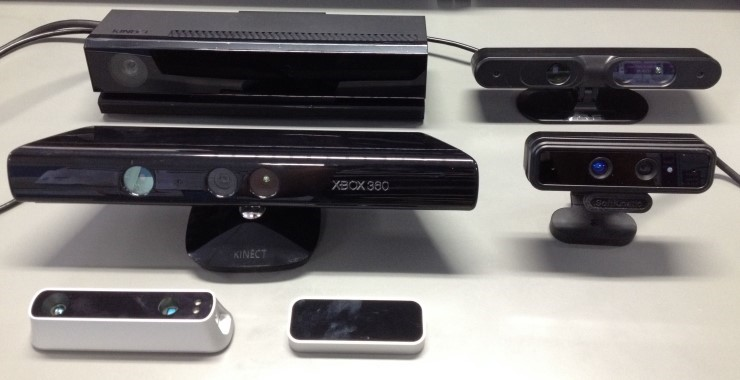
\includegraphics[width=0.7\columnwidth]{pictures/chapter9/depth_camera.jpg}
\caption{Depth cameras}
\end{figure}

그 방식이 다르던, PCD 데이터를 받는다는 점에서 LRF 를 포함한 Depth Sensor 계열을 동일하다. 우선, 이 강좌에서는 위 그림 오른쪽 맨위에 있는 Asus의 Xtion을 이용하기로 하겠다. 

\setcounter{num}{0}

\vspace{\baselineskip}
\noindent
\stepcounter{num}
\thenum) 우선, ROS의 OpenNI 관련 패키지를 다운로드/설치 한다.

\begin{lstlisting}[language=ROS]
sudo apt-get install ros-indigo-openni2-camera ros-indigo-openni2-launch
\end{lstlisting}

\vspace{\baselineskip}
\noindent
\stepcounter{num}
\thenum) Xtion 을 구입하게 되면 동봉된 CD에 Xtion 드라이브가 있다. 함께 설치해주도록 하자.

\begin{lstlisting}[language=ROS]
tar -xvf Sensor-Bin-Linux-x64-v5.1.0.41.tar.bz2
cd Sensor-Bin-Linux-x64-v5.1.0.41/
sudo sh install.sh 
\end{lstlisting}

\vspace{\baselineskip}
\noindent
\stepcounter{num}
\thenum) ROS의 Openni2 런치 파일을 실행시켜주자.

\begin{lstlisting}[language=ROS]
$ roscore
$ roslaunch openni2_launch openni2.launch
\end{lstlisting}

%-------------------------------------------------------------------------------
\subsection{Point Cloud 정보값 확인}

\setcounter{num}{0}

\stepcounter{num}
\thenum) RViz 실행

\begin{lstlisting}[language=ROS]
$ rosrun rviz rviz
\end{lstlisting}

\vspace{\baselineskip}
\noindent
\stepcounter{num}
\thenum) Displays 옵션 변경

\vspace{\baselineskip}
\noindent
\thenum-1) Fixed Frame 변경
Global Options → Fixed Frame 을 "camera\_depth\_frame" 로 변경한다.

\vspace{\baselineskip}
\noindent
\thenum-2) PointCloud2 추가 및 설정
rviz 좌측 하단의 Add 클릭한 후, PointCloud2를 선택하여 추가한다. 아래 그림과 같이 세부 설정을 바꿔준다.

\begin{figure}[h]
\centering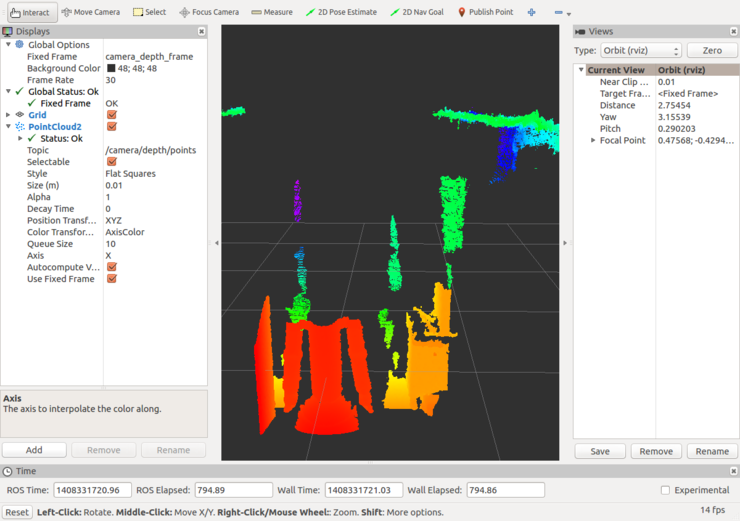
\includegraphics[width=0.9\columnwidth]{pictures/chapter9/rviz_pc2.png}
\caption{RViz PointCloud2 디스플레이}
\end{figure}

\vspace{\baselineskip}
\noindent
\stepcounter{num}
\thenum) 데이터 확인

위 그림과 같이, PCD 값을 확인할 수 있다. 현재, 색을 X축을 기준으로 하였기에 X축을 기준으로 멀어질 수록 보라색에 가깝게 된다.

%-------------------------------------------------------------------------------
\subsection{Depth camera 활용}

Depth camera의 활용은 무궁무진 할테지만 대표적인 예는 점군 데이터를 이용한 SLAM (Simultaneous localization and mapping) 이라고 할 수 있다. 굳이 SLAM이 아니더라도 모바일 로봇이나 무인 자동차에도 많이 사용되고 있다. 또한, 사람의 골격 정보를 이용하여 로봇과의 상호작용인 HRI 에도 많이 사용된다. 예를들어 아래의 동영상과 같은 것이 있는데 모두가 Depth camera 를 이용한 모션캡쳐, 로봇 조정, 제스처를 통한 이동 포인트 지정 등이 있다. 이 부분에 대해서는 추후에 강좌를 통해서 소개하도록 하겠다.






%-------------------------------------------------------------------------------
